\section{Esempio di grafo reale}
Per analizzare meglio il sistema Bitcoin, viene creato un grafo delle transazioni, utilizzando dei dati reali. Nella \textit{figura \ref{fig:txgraph}} è visualizzato il grafo generato dall'elaborazione solo di 5 blocchi, in particolare dal blocco 417113 al 417117.

\begin{figure}[htbp]
	\centering
	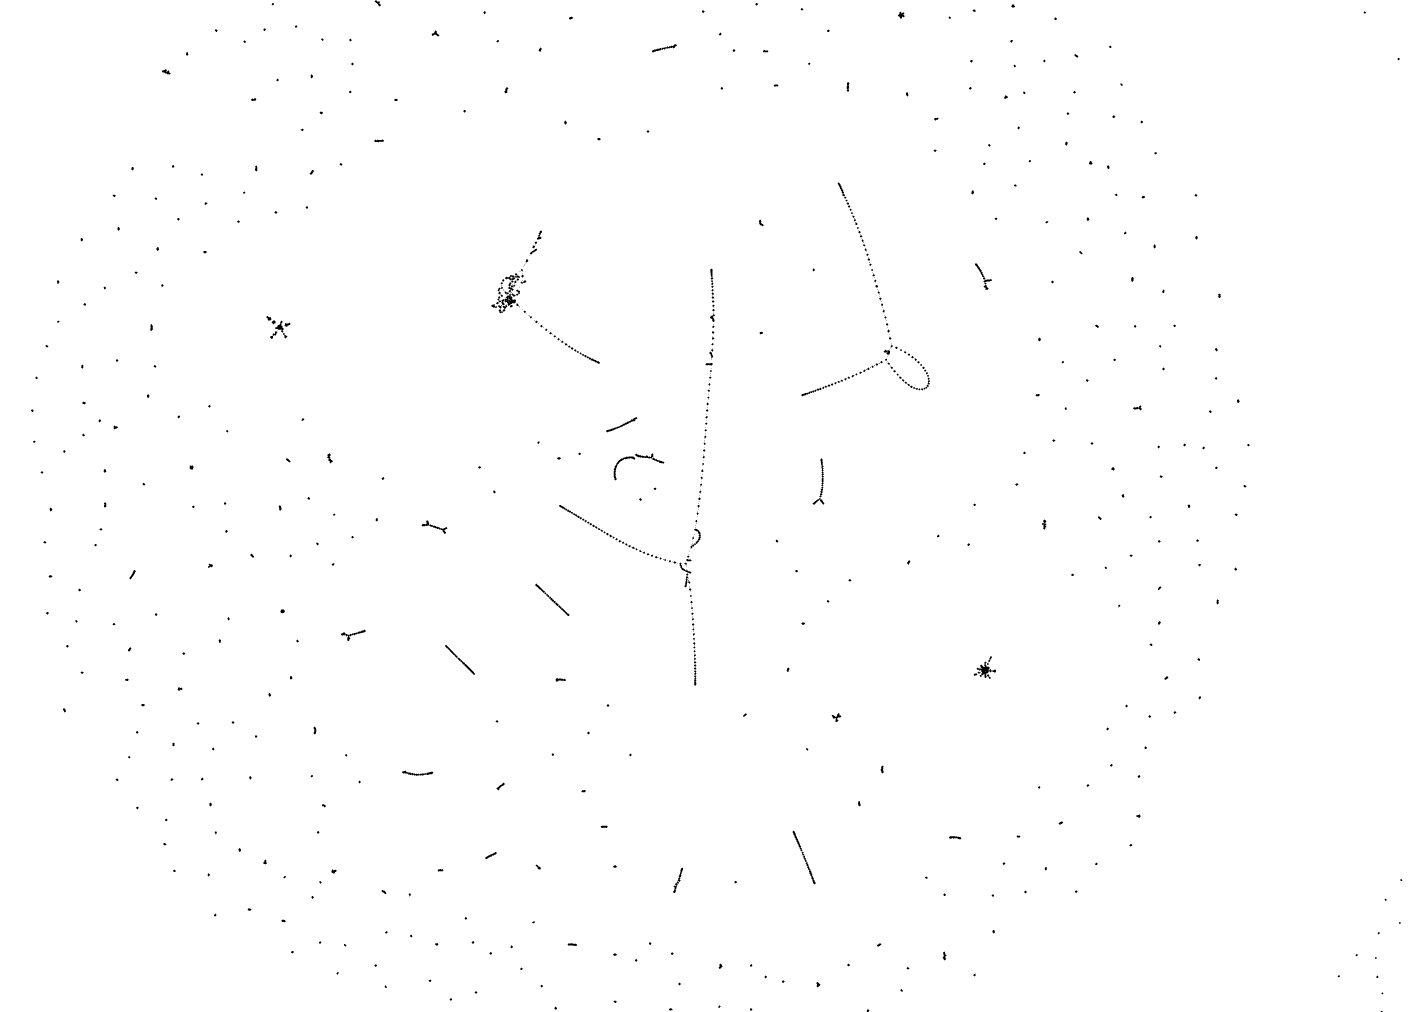
\includegraphics[width =0.8 \linewidth]{figure/txgraph}
	\caption{\textit{Esempio di tx-graph reale}}\label{fig:txgraph}
\end{figure}

Tale grafo viene visualizzato utilizzando il metodo \textit{force-directed}, ovvero assegnando ad ogni arco delle forze attrattive in modo da disporre i nodi del grafo.
A colpo d'occhio, al centro dell'immagine si notano alcune linee, che rappresentano delle sequenze di nodi collegati tra loro uno dopo l'altro.
Guardando man mano verso l'esterno, si notano molti nodi scollegati dal grafo: molto probabilmente rappresentano transazioni i cui output non sono stati spesi in transazioni incluse nell'intervallo di blocchi considerato, oppure che non sono stati spesi affatto.

\section{Lunghe catene di transazioni}
La media del numero di transazioni Bitcoin giornaliere è all'incirca 280'000, valutato a Maggio 2017. Questo numero è conosciuto per essere largamente influenzato da alcuni fenomeni.
Il mescolamento dei wallets e il mixing dei soldi sono solamente due esempi di attività che generano transazioni le quali non sono direttamente collegate con il reale acquisto di beni o servizi. Un altro esempio viene dall'attività di alcuni \textit{exchange}(organizzazioni che permettono agli utenti di scambiare Bitcoin per la valuta legale e viceversa) che usano lunghe catene di transazioni per emettere pagamenti verso degli utenti che hanno deciso di ritirare i Bitcoin. 

Questo tipo di organizzazioni aggregano diversi depositi di bitcoin dentro una singola grande transazione.  Sebbene tali catene di transazioni vengono innescate da attività umane (per esempio utenti che decidono di scambiare bitcoin), esse sono comunque generate da un meccanismo automatico, il quale incrementa il numero giornaliero delle transazioni associate al commercio esplicito di beni o servizi tra utenti.

Sulla base di ciò, si pensa che le organizzazioni con interessi sui Bitcoin, generano transazioni con il mero obiettivo di attrarre investitori e incrementare il tasso di scambio. Essendo generate da software, queste transazioni "artificiali" spesso introducono dei pattern regolari all'interno della Blockchain. E tali pattern vengono generati proprio perchè le catene di transazioni sono generate da un software programmato. 

Queste considerazioni vengono trattate approfonditamente nel paper \cite{ddp-ltcbh-17}. L'argomento principale di tale documento è il parametro \textit{LLC}, acronimo di \textit{lenght of the longest chain}, ovvero "lunghezza della catena più lunga". Ogni transazione viene etichettata con un LLC, ovvero un numero che rappresenta la catena più lunga a cui appartiene la transazione. Per assegnare questo parametro, viene precedentemente effettuata un'analisi sul grafo delle transazioni. Quindi, per ogni transazione, ovvero per ogni nodo, viene calcolato l'LLC e assegnato alla singola transazione. Infine vengono fatte delle analisi sui dati e sulla distribuzione del parametro rispetto ai blocchi considerati nell'esecuzione dell'algoritmo.

Capire se una chain di transazioni è stata generata automaticamente o riflette una chain creata da acquisti reali di umani, è una sfida stimolante. Infatti, la \textit{chain of ownership} ("catena di proprietà") introduce naturalmente lunghe chain di transazioni nel tx-graph. Quello che non è naturale è la velocità con cui tali chain vengono generate. 
